%
% File naaclhlt2015.tex
%


\documentclass[11pt,letterpaper]{article}
\usepackage{naaclhlt2015}
\usepackage{times}
\usepackage{latexsym}
\usepackage{amsmath}
\usepackage{amssymb}
\usepackage{tikz}
\usepackage{multirow}

\usepackage{tikz-qtree}
\usepackage{tikz-dependency}
\usepackage{proof}
\usepackage{fullpage}
\usepackage{todonotes}
\usepackage{multicol}

\newtheorem{theorem}{Theorem}[section]
\newtheorem{lemma}[theorem]{Lemma}
\newtheorem{proposition}[theorem]{Proposition}
\newtheorem{corollary}[theorem]{Corollary}

\newenvironment{proof}[1][Proof]{\begin{trivlist}
\item[\hskip \labelsep {\bfseries #1}]}{\end{trivlist}}
\newenvironment{definition}[1][Definition]{\begin{trivlist}
\item[\hskip \labelsep {\bfseries #1}]}{\end{trivlist}}
\newenvironment{example}[1][Example]{\begin{trivlist}
\item[\hskip \labelsep {\bfseries #1}]}{\end{trivlist}}
\newenvironment{remark}[1][Remark]{\begin{trivlist}
\item[\hskip \labelsep {\bfseries #1}]}{\end{trivlist}}

\newcommand{\qed}{\nobreak \ifvmode \relax \else
      \ifdim\lastskip<1.5em \hskip-\lastskip
      \hskip1.5em plus0em minus0.5em \fi \nobreak
      \vrule height0.75em width0.5em depth0.25em\fi}

\usepackage[font=footnotesize]{caption}
\usepackage{amsfonts}
\usepackage{amsmath}
\DeclareMathOperator*{\argmax}{arg\,max}
\DeclareMathOperator*{\argmin}{arg\,min}

\usepackage{algpseudocode}
\usepackage{algorithm}

\usetikzlibrary{arrows}
\usetikzlibrary{decorations.markings}
\tikzset{
  >=latex,text height=1.5ex,text depth=0.25ex
}

\newcommand{\nonterms}{\mathcal{N}}
\newcommand{\END}{\mathrm{END}}
\newcommand{\START}{\mathrm{START}}
\newcommand{\rules}{\mathcal{R}}
\newcommand{\terms}{\mathcal{T}}
\newcommand{\Left}[1]{#1_{\Leftarrow}}
\newcommand{\Right}[1]{#1_{\Rightarrow}}
\newcommand{\Span}[1]{\langle #1 \rangle}
\newcommand{\tri}{\langle \Left{m}, \Right{m} \rangle}

\newcommand{\Tag}[1]{\texttt{#1}}
\newcommand{\Root}{r}

\newcommand{\RuleSym}{\mathrm{rule}}
\newcommand{\Rule}[3]{#1 \rightarrow #2\ #3}
\newcommand{\RuleA}[3]{#1 \rightarrow #2^*\ #3}
\newcommand{\RuleB}[3]{#1 \rightarrow #2\ #3^*}
\newcommand{\BinFN}[1]{\mathrm{bin}({#1})}
\newcommand{\TagFN}[1]{\mathrm{tag}({#1})}
\newcommand{\WordFN}[1]{x_{#1}}
\newcommand{\Reals}{\mathbb{R}}
\newcommand{\ParseName}{\textsc{ParPar}}

\newcommand{\smrcomment}[1]{\textcolor{green}{\bf \small [#1 --smr]}}
\newcommand{\lpkcomment}[1]{\textcolor{red}{\bf \small [#1 --lpk]}}
\newcommand{\nascomment}[1]{\textcolor{blue}{\bf \small [#1 --nas]}}


\setlength\titlebox{6.5cm}    % Expanding the titlebox

\title{Parsing Dependencies}

\author{}
% \author{Author 1\\
% 	    XYZ Company\\
% 	    111 Anywhere Street\\
% 	    Mytown, NY 10000, USA\\
% 	    {\tt author1@xyz.org}
% 	  \And
% 	Author 2\\
%   	ABC University\\
%   	900 Main Street\\
%   	Ourcity, PQ, Canada A1A 1T2\\
%   {\tt author2@abc.ca}}


%% For drawing the traps/tris.

\date{}

\begin{document}
\maketitle
\begin{abstract}
We present a new algorithm for transforming dependency parse trees into
phrase-structure parse trees.  We cast the problem as  structured
prediction and learn a statistical model.  Our algorithm is faster than traditional
phrase-structure parsing and achieves accuracy near to the state of
the art on English and Chinese benchmarks.

  % Motivated by the increase in accuracy of statistical dependency
  % parsers, we consider the problem of decoding phrase-structure parses
  % directly from predicted dependency trees. Unlike past rule-based
  % approaches, we treat this as a structured prediction problem using a
  % specialized context-free parser. Since our parser makes use of the
  % predicted dependency structure it is asymptotically faster and much
  % simpler than a standard lexicalized parser. However, despite its
  % simplicity, it still yields high-accuracy phrase-structure parses on
  % experiments in both English and Chinese.



\end{abstract}

\section{Introduction}

\nascomment{rewrote the intro.  I think the paper will be more
  exciting if, instead of making claims about informativeness or
  suggesting preferences, we just say the way the world turned out, and then
  ask how things might have turned out if it had been different.}

Natural language parsers typically produce phrase-structure (or
constituent) trees or dependency trees.  These representations capture
some of the same syntactic phenomena, and the two can be produced
jointly \cite{carreras2008tag,rush2010dual}.  Yet it
appears to be completely unpredictable which will be preferred by a
particular application.  Both continue to receive the attention of
parsing researchers.


Further, it appears to be a historical accident that phrase-structure
syntax was used in annotating the Penn Treebank, and that English
dependency annotations are largely derived through mechanical,
rule-based transformations applied to the Penn Treebank.  Indeed,
despite extensive work on direct-to-dependency parsing algorithms
(which we call \emph{d-parsing}), the most accurate dependency
parsers for English still involve phrase-structure parsing (which we
call \emph{c-parsing}) followed by rule-based extraction of
dependencies \cite{kong2014empirical}.
 % \nascomment{could reference the table here, or
 %  just cite}.

What if dependency annotations had come first?  Because d-parsers are
generally much faster than c-parsers, we consider an alternate
pipeline: d-parse first, then transform the dependency representation
into a phrase-structure tree constrained to be consistent with the
dependency parse.  This idea was explored by  \newcite{xia2001converting} and
\newcite{xia2009towards} using hand-written rules.  Here we present a data-driven
algorithm in the structured prediction framework.  The approach can be
understood as a pipeline, or as a specially-trained coarse-to-fine
decoding algorithm where a d-parser provides ``coarse'' structure and
the second stage refines it \cite{??}.

Our lexicalized phrase-structure parser is
asymptotically faster than
  parsing with a lexicalized context-free grammar:  $O(n^2)$ plus
  d-parsing,
  vs.~$O(n^5)$ worst case runtime in sentence length $n$, with the same grammar constant.
   With simple pruning, our approach achieves
  linear observable runtime.  The accuracy of the approach is similar
  to state-of-the-art phrase-structure parsers without reranking or
  semisupervised training.


\nascomment{I suggest giving a brief roadmap here, or (better) integrating it
  into the discussion above}



% There are two main grammatical
% frameworks used for statistical syntactic prediction: phrase-structure parsers and
% dependency parsers \cite{}. The two offer a
% trade-off: phrase-structure parsing is very accurate \lpkcomment{i am not sure if the accurate is the right word here... dep parser is also very accuarate.} and provides a
% full context-free syntactic representation; dependency parsing is
% often faster, but still
% predicts much of the useful\lpkcomment{again... here i think maybe we should say different rather than imply which is more useful?} syntactic structure.

% We can quantify this difference by looking
% at the dependency prediction accuracy of phrase-structure parsers. Table~\ref{fig:depcomp} shows this comparison across several widely-used parsers. Note that the best models are phrase-structure parsers, but that recent advances in dependency parsing have led to comparably high-accuracy dependency parsers.\lpkcomment{this is a little confusing? there are two ways to get dependencies, c-parsing and d-parsing, but here it seems we are comparing the acc between phrase-structure and dependency parsing acc? they are two different systems....}

% The natural reverse question is how well do these dependency parsers perform at phrase-structure prediction? Is it reasonable to use dependency parsers for tasks that require phrase-structure trees as input? \lpkcomment{i would like to put the benefits of doing this dep2phrase thing in the intro maybe? 1) it is very fast since dep prunes away a lot not useful cky chart item 2) dep can server as features in this problem, so that we can aim at higher acc with easy cky model. (actually, i believe the dep parsers can see syntactical information which is not easy to see when using cky, that's also the reason why your phrase+dep decomposition works right?)}

% \nascomment{someone else's rewrite:}

% Statistical dependency parsers provide a fast and accurate method for
% predicting syntactic structure; however, many applications of parsing still rely on
% full phrase-structure trees, and cannot use parsers that only predict
% dependency structure. 

% In this work we present a new parser, \ParseName, that takes dependency trees as input and produces phrase-structure trees as output. The parser has several advantages

% \begin{itemize}
% \item Accuracy; The parser is as accurate as several widely-used phrase-structure parsers \%.  
% \item Efficiency; Asymptotically it is much faster than standard phrase-structure parsers; empirically it is as fast an efficient dependency parser.

% \item Flexibility; The parser only requires dependencies at test-time, and so it can improve alongside dependency parsers.
% \end{itemize}

% Recovering the best phrase-structure tree is a non-trivial problem. Given a
% predicted dependency tree, there is a large space of possible output
% phrase-structure trees, each tree may have many possible labelings,
% and there are likely errors in the input dependency tree. Figure~\ref{fig:inverse} shows the possible unlabeled trees for a single dependency tree input.

\begin{figure}
  \centering

  \vspace{-1cm}

  \begin{dependency}[theme=simple]
    \begin{deptext}[column sep=0.7cm]
      I$_1$ \& saw$_2$ \& the$_3$ \& man$_4$ \\
    \end{deptext}
    \deproot{2}{ROOT}
      \depedge{2}{1}{}
      \depedge{4}{3}{}
      \depedge{2}{4}{}
  \end{dependency}

  \scalebox{0.7}{
    \Tree [ .X(2) [ .X(1) [ .N I$_1$ ] ]  [ .V saw$_2$ ] [ .X(4) [ .D the$_3$ ]  [ .N man$_4$ ] ] ]
    \Tree [ .X(2)  [ .N I$_1$ ] [ .X(2)  [ .V saw$_2$ ] [ .X(4) [ .D the$_3$ ]  [ .N man$_4$ ] ] ] ]
    \Tree [ .X(2) [ .X(2) [ .N I$_1$ ]   [ .V saw$_2$ ] ]  [ .X(4) [ .D the$_3$ ]  [ .N man$_4$ ] ] ]
  }
  \label{fig:inverse}
  \caption{{\footnotesize 
      % While a phrase-structure parse determines a
      % unique dependency parse \nascomment{only given head rules!  misleading}, the inverse problem is
      % non-deterministic.
      It is standard to transform c-parses to d-parses using deterministic head rules.
      The figure, adapted from
      \cite{collins1999statistical}, shows several X-bar trees that
      all produce the same dependency structure. The parentheses
      $X(h)$ indicate the head $h$ of each internal vertex. }
    }
\end{figure}


% Unfortunately, as illustrated in Figure~\ref{fig:inverse},
% recovering the best phrase-structure tree is a non-trivial problem. Given a
% predicted dependency tree, there is a large space of possible output
% phrase-structure trees, each tree may have many possible labelings,
% and there are likely errors in the input dependency tree.



% In this work, we pose phrase-structure recovery as a structured
% prediction problem, and train a full lexicalized phrase-structure
% parser, \ParseName,  to predict the syntactic tree for a given sentence. Crucially,
% though, we limit the search space of the parser to the search space
% that produces a given dependency tree. We show that,
% To handle these issues, our system poses phrase-structure recovery  as a structured
% prediction problem, and uses a lexicalized phrase-structure
% parser to predict the best tree. Crucially,
% though, the search space of the parser is limited by the dependency tree, 
% which keeps the underlying parser simple and the system efficient.






% \begin{table}
%   \centering
%   \small
%   \begin{tabular}{|l|l|r|}
%     \hline
%     Type & Model & UAS  \\
%     \hline

%     \hline
%     \multirow{4}{*}{Phrase Structure} & Petrov[06] & 92.66   \\
%     & Stanford PCFG & 88.88 \\
%     & CJ Reranking & 93.92 \\
%     & Stanford RNN & 92.23 \\
%     \hline
%     \multirow{1}{*}{Dependency} & TurboParser & 93.59  \\
%     \hline
%   \end{tabular}
%   \caption{Dependency accuracy for several several widely used phrase-structure and dependency parsers.
%     Score are reported as the unlabeled accuracy score (UAS) of dependencies on PTB  Section 22.
%     Conversion are performed using the Collins head rules \cite{collins2003head}.
%     Note that the best scoring is a reranking phrase-structure parser, but that state-of-the-art
%     dependency parsers are comparable with the best parsers.
%     \nascomment{not sure this is worth keeping; could just make the
%       point and cite Kong and Smith 2014 arXiv paper.}}
%   \label{fig:depcomp}
% \end{table}




\section{Background}

We begin by developing notation for a c-parsing, using a lexicalized context-free grammar, and for d-parsing. The notation aims to highlight the similarity between the two formalisms.

\subsection{Lexicalized CFG Parsing}

A lexicalized context-free grammar (LCFG) is a context-free grammar 
paired with a set of head rules. Define an binarized\footnote{For notational simplicity we ignore unary rules for this section.} LCFG as a 4-tuple $(\nonterms, \rules, \terms, \Root)$ where:
\begin{itemize}
\item $\nonterms$; a set of nonterminal symbols, e.g. \Tag{NP}, \Tag{VP}.
\item $\terms$; a set of terminal symbols, consisting of the words in the language.
\item $\rules$; a set of lexicalized rule productions either of the form $\RuleA{A}{\beta_1}{\beta_2}$ or $\RuleB{A}{\beta_1}{\beta_2}$  consisting of a parent nonterminal $A \in \nonterms$, a sequence of children $\beta_i \in \nonterms \cup \terms$ for $i \in \{1, 2\}$, and a distinguished head child annotated with $*$. The head child comes from the head rules associated with the grammar.
\item $\Root$; a distinguished root symbol $\Root \in \nonterms$.
\end{itemize}

Given an input sentence $x_1, \ldots, x_n$ of terminal symbols from $\terms$, define $\mathcal{Y}(x)$ as the set of c-parses for the sentence. This set consists of all binary ordered trees with fringe $x_1, \ldots,  x_n$, internal nodes labeled from $\nonterms$, all tree productions  $A \rightarrow \beta$ consisting of members of $\rules$, and root label $\Root$.


For a c-parse $y \in \mathcal{Y}(x)$,
we further associate a triple $v = (\Span{i, j}, h, A)$ with each vertex in the tree, where



\begin{itemize}
\item $\Span{i,j}$; the \textit{span}  of the vertex, i.e. the contiguous sequence $\{x_i, \ldots, x_j\}$ of the sentence covered by the vertex.

\item $h(v) \in \{1, \ldots, n\}$; index indicating that $x_h$ is the \textit{head} of the vertex, defined recursively by the following rules:
  \begin{enumerate}
  \item  If the vertex is leaf $x_i$, then $h=i$.
  \item Otherwise,  $h$ matches the head child where $\RuleA{A}{\beta_1}{\beta_2}$ or $\RuleB{A}{\beta_1}{\beta_2}$  is the rule production at this vertex.
  \end{enumerate}

\item $A \in \terms \cup \nonterms$; the terminal or nonterminal symbol of the vertex.
\end{itemize}

Note that all but one word $x_i$ has an ancestor vertex $v$ where $h(v) \neq i$.  Define the
\textit{spine} of word $x_i$ to be the longest of chain connected vertices $v_1,
\ldots, v_p$ where $h(v_j) = i$ for $j \in \{1, \ldots, p\}$.
Also if it exists, let vertex $v_{p+1}$  be the parent of vertex~$v_p$,
where $h(v_{p+1}) \neq i$. The full notation is illustrated in Figure~\ref{fig:spine}.

\begin{figure}
  \centering


  \Tree [ .\node[color=red]{$(\Span{1,n}, 3, \Tag{S})$}; [ .\node[color=blue]{$(\Span{1,2}, 2,  \Tag{NP})$}; [  .\node{$(\Span{1,1}, 1,  \Tag{DT})$}; The$_1$ ]  [ .\node[color=blue]{$(\Span{2,2}, 2, \Tag{NN})$}; \textcolor{blue}{automaker$_2$} ] ] [ .\node{$(\Span{3,3}, 3,  \Tag{VBD})$}; sold$_3$ ] [ .\node{..}; ] ]



  \begin{dependency}[theme=simple]
    \begin{deptext}[column sep=0.7cm]
      The$_1$ \& automaker$_2$ \& sold$_3$ \& $\ldots$ \\
    \end{deptext}
    \deproot{3}{}
      \depedge{2}{1}{}
      \depedge{3}{2}{}
  \end{dependency}


  % \Tree [ .A [ .B  C ] ]
  \caption{Figure illustrating an LCFG parse. The parse is an ordered tree with fringe $x_1, \ldots, x_n$. Each vertex is annotated with a span, head, and syntactic tag. The blue vertices represent the 3-vertex spine $v_1, v_2, v_3$ of the word \texttt{automaker$_2$}. The root vertex is $v_4$, which implies that \texttt{automaker$_2$} modifies \texttt{sold$_3$} in the induced dependency graph.     }
  \label{fig:spine}
\end{figure}

\subsection{Dependency Parsing}

Dependency trees provide an alternative, and in some sense simpler,
representation of grammatical structure.


For sentence $x_1,
\ldots, x_n$, define a d-parse $d$ as a sequence $d_1, \ldots, d_n$ where for all $i$, $d_i \in \{0, \ldots, n\}$. These dependency relations can be seen as arcs $(d_i, i)$ in a directed graph over the sentence, where $x_0$ is a special pseudo-root vertex.  A dependency parse is valid  if the corresponding directed graph is a directed tree rooted at vertex~$0$. Figure~\ref{fig:spine} contains an example of a d-parse.

For a valid dependency tree, define the \textit{span} of any word $x_m$ as the set of indices reachable from vertex $m$ in the directed tree. A dependency parse is \textit{projective} if the descendants of every word in the tree form a contiguous span of the original sentence \cite{}. We use the notation $\Left{m}$ and $\Right{m}$ to represent the left- and
right-boundaries of this span.


Any lexicalized c-parse can be converted to a unique projective d-parse.
For an input symbol $x_m$ with spine $v_1, \ldots, v_p$,

\begin{enumerate}
\item If $v_p$ is the root of the tree,
then $d_m = 0$.
\item Otherwise let $v_{p+1}$ be the parent vertex of
$v_p$ and $d_m = h(v_{p+1})$. The span $\Span{i, j}$ of $v_p$ in the lexicalized c-parse is equal to  $\Span{\Left{m}, \Right{m}}$
in the  d-parse.
\end{enumerate}


However the conversion from d-parse to c-parse tree is more challenging, and in fact, it can be shown that in the worst-case there are an
exponential number of possible unlabeled phrase-structure trees that induce the same dependency parse (proof given in Appendix~\ref{app:proof}).


\section{Parsing Dependencies}

The aim of this work is to predict the best c-parse
from a given d-parse. Since this problem is ill-posed,
we will learn a function to score possible c-parses
and generate the highest-scoring parse. In this section
we assume we have this function and discuss the prediction
problem. We return to training in the next section.



% Since the inverse problem is ill-posed, our goal will
% be to learn a scoring function to help predict a
% phrase-structure tree for any dependency parse. In
% this section we assume this function is given and describe
% the prediction problem. In the next section we consider
% the learning problem.


\begin{figure*}
  \begin{multicols}{2}
  \noindent \textbf{Premise:}
  \[(\Span{i, i}, i, A)\ \ \ \forall i \in \{1 \ldots n\}, A \in {\cal N}\]

  \noindent\textbf{Rules:}

   For $i\leq h \leq k < m \leq j$,  and  rule  $\RuleA{A}{\beta_1}{\beta_2}$,
   \[\infer{( \Span{i, j},  h,  A)}{( \Span{i, k}, h, \beta_1)  &  ( \Span{k+1, j}, m, \beta_2) } \]

   For $i\leq m \leq k < h \leq j$, rule  $\RuleB{A}{\beta_1}{\beta_2}$,
   \[\infer{(\Span{i, j},  h, A)}{(\Span{i, k}, m, \beta_1)  &  (\Span{k+1, j}, h, \beta_2) }  \]

\noindent \textbf{Goal:}
\[ (\Span{1, n}, m, \Root) \mathrm{\ for\ any }\ m\]

\label{fig:cky}

  \noindent \textbf{Premise:}
  \[(\langle i,i \rangle, i, A)\ \ \ \forall i \in \{1 \ldots n\}, A \in {\cal N}\]

  \noindent\textbf{Rules:}

  For all   $i < m, h = d_m$  and rule  $\RuleA{A}{\beta_1}{\beta_2}$,
  \[\infer{( \Span{i, \Right{m}}, h, A)}{(\Span{i, \Left{m}-1}, h, \beta_1)  &  (\tri, m, \beta_2) } \]

  For all    $m < j, h = d_m$ and  rule  $\RuleB{A}{\beta_1}{\beta_2}$,
  \[ \infer{( \Span{ \Left{m}, j }, h, A)}{(\tri, m, \beta_1)  &  (\Span{\Right{m}+ 1, j}, h, \beta_2) } \]

\noindent \textbf{Goal:}
\[(\Span{1, n}, m, \Root) \mathrm{\ for\ any }\ m \mathrm{\ s.t. \ } d_m = 0 \]

\end{multicols}
\label{fig:cky_new}
\caption{The two algorithms written as deductive parsers. Starting from the \textit{premise}, any valid application of \textit{rules} that leads to a \textit{goal} is a valid parse.  (a) Lexicalized CKY algorithm for LCFG parsing. For this algorithm there are $O(n^5|\rules|)$ rules where $n$ is the length of the sentence. (b) The constrained CKY parsing algorithm for $\mathcal{Y}(x, d)$. The algorithm is nearly identical except that many of the free indices are now fixed to the dependency parse. Finding the optimal parse is now $O(n^2|\rules|)$.}
\end{figure*}

\subsection{Constrained Parsing Algorithm}


Our prediction algorithm will be a simple extension of the standard lexicalized CKY parsing algorithm.

Assume that we are given a binarized LCFG defining a set of valid c-parses $\mathcal{Y}(x)$.
The parsing problem is to find the highest-scoring parse in this set, i.e.  \[ \hat{y} \gets \argmax_{y \in {\cal Y}(x)} s(y;x) \] where
$s$ is a scoring function.

We further assume that scoring function factors over rule productions, 
and so the highest-scoring parse can be found using the lexicalized
CKY algorithm. This algorithm is defined deductively
in Figure~\ref{fig:cky_new}. The productions are of the form

\[ \infer{(\Span{i, j}, h, A)}{(\Span{i, k}, m, \beta_1) & (\Span{k+1,
    j}, h, \beta_2)} \] for all rules $\RuleB{A}{\beta_1}{\beta_2}\in
\rules$ and spans $i \leq k < j$. This particular production indicates that
rule $\RuleB{A}{\beta_1}{\beta_2}$ was applied at a vertex covering
$\Span{i, j}$ to produce two vertices covering $\Span{i, k}$ and
$\Span{k+1, j}$, and that the new head is index $h$ which is modified
by index $m$.

The highest-scoring parse can found by bottom-up dynamic programming
over these productions, and the running time is linear in the number
of production. The standard lexicalized CKY algorithm requires $O(n^5
|\rules|)$ time, which is intractable to run without heavy pruning.

 Fortunately, the parsing problem becomes much simpler if 
 we are constrained to a given d-parse, $d_1, \ldots, d_n$.
 Define the set $\mathcal{Y}(x,d)$ as all valid LCFG parses that map
 to this dependency parse (as defined in the previous section). 
  Our aim is to find

\[ \argmax_{y \in \mathcal{Y}(x, d)} s(y; x, d)\]

This new problem has a nice property. For any word $x_m$ with spine $v_1, \ldots, v_p$ the LCFG span  $\Span{i,j}$ of $v_p$ is equal to the dependency span $\Span{\Left{m},\Right{m}}$ of $x_m$. These dependency spans can be efficiently computed directly from the dependency parse $d$.

This property greatly limits the search space of the parsing problem.
Instead of searching over all possible spans $\Span{i, j}$ of each modifier, we can
precompute $\langle \Left{m},\Right{m}\rangle$. Figure~\ref{fig:cky_new} shows the new algorithm.
While the productions are the same as the original algorithm, there are many fewer of them. 
There is one production for each index and each possible modifier, leading to an algorithm with $O(n^2|\rules|)$ running time.


% \subsection{Further Pruning}
% \label{sec:prune}

Finally in addition to constraining the topology of c-parses, we
also experiment with pruning to limit the space of rules. 
We observe that in training the part-of-speech of the head word $x_h$
greatly limits the possible rules $\Rule{A}{\beta_1}{\beta_2}$.  To
exploit this property we build tables $\rules_t$ for each
part-of-speech tag $t$ and limit the search to rules seen for the
current head tag.

An important concern is whether it is even possible to recover
c-parses under these constraints. To answer this question we ran
oracle experiments to find the best c-parse possible under each
algorithm.  Table~\ref{tab:alg-oracle} shows a
comparison among full LCFG parsing, dependency limited parsing, and
dependency-limit pruned parsing. These experiments show that there 
is a sizable drop in oracle accuracy with the d-parse constraints, but that
the upper-bound on accuracy is still high enough to make this task interesting. 

% Full LCFG is very slow, even on very
% short sentences.  Limiting to dependency structures leads to a large
% speed up, but a drop in oracle score. Pruning gives a further speed
% up, without hurting oracle performance.




\begin{table}
  \centering
  \small
  \hspace*{-0.3cm}
  \begin{tabular}{|l|ccrr|}
    \hline
    Model & Sym & Comp. & Speed & Oracle  \\
    \hline
    \hline
    LCFG($< 20$)  & $\mathcal{Y}(x)$ & $O(n^5|\rules|)$ &     0.25 & 100.0  \\
    LCFG(dep)    & $\mathcal{Y}(x,d)$ & $O(n^2|\rules|)$ &  63.2 & 92.8    \\
    LCFG(prune)  &  - & $O(n^2|\rules|)$ &   173.5 & 92.7 \\
    \hline
  \end{tabular}
  \label{tab:alg-oracle}
  \caption{Comparison of three parsing setups:
    LCFG($<20$) is the standard full lexicalized grammar limited to sentence of length
    less than 20 words, LCFG(dep) is
    limited to the dependency skeleton, and LCFG(prune) is the pruning described in
    Section~\ref{sec:prune}. \textit{Oracle} is the oracle f-score on the development data (described in Section~\ref{sec:analysis}). \textit{Speed} is the efficiency of the parser on development data in sentences per second.}
\end{table}

\subsection{Binarization}

\smrcomment{This section is wrong, start over}

% So far we have assumed the grammar is binarized, we must convert the
% non-binary treebank grammars to binary form.  
To this point we have assumed the grammar is binarized, 
While the algorithm
itself is not dependent on the binarization used, this choice affects
the run-time of the algorithm, through $\rules$, as well as the
structure of the scoring function.

% Our binarization decomposes non-binary rules into fragments for
% each head-modifier pair.

For simplicity, we consider binarizing rule $\langle A \rightarrow \beta_1 \ldots \beta_m,
k\rangle$ with $m > 2$. Relative to the head $\beta_k$
the rule has left-side $\beta_1 \ldots \beta_{k-1}$ and right-side
$\beta_{k+1} \ldots \beta_m$.

We replace this rule with binary rules that consume each side
independently as a first-order Markov chain (horizontal Markovization).
The main transformation is to introduce rules

\begin{itemize}

\item
$\Rule{A^{|}}{A^{|*}}{\beta_i}$ for $k < i < m$

\item
$\Rule{A^{|}} {\beta_i}{A^{|*}} $ for $1< i < k$
\end{itemize}


% As an example consider the rule

Additionally we introduce several additional rules to handle the boundary cases of starting a new rule, finishing the right side, and completing a rule. (These rules are slightly modified when $k\leq 2$ or $k=m$).
\begin{align*}
& \RuleA{A^{\Rightarrow}_{\beta_{k+1}}}{\beta_k}{\beta_{k+1}} & \Rule{A^{\Rightarrow*}} {A^{\Rightarrow}_{\beta_{m-1}}}{\beta_m} \\
 &\Rule{A^{\Leftarrow}_{\beta_{k-1}}}{\beta_{k-1}}{A^{\Rightarrow *}} & \Rule{A}{\beta_1}{ A^{\Leftarrow*}_{\beta_{2}}}\\
\end{align*}

\noindent For example the transformation of a common rule looks like

\begin{center}
  \scalebox{0.6}{ \Tree [ .S NP VP$^*$ NP NP ] $\Rightarrow$ \Tree [
    .S NP [ .S$^{\Rightarrow*}$ [ .S$^{\Rightarrow*}_{NP}$ VP$^*$ NP ]
    NP ] ] }
\end{center}

\noindent Each rule contains at most 3 original nonterminals so the size of the new binarized rule set is bounded by $O(\nonterms^3)$.



\section{Structured Prediction}

To learn the scoring function for the transformation from d-parses to c-parses,
we use a standard structured prediction setup.
Define the scoring function $s$ as

\[s(y;x, d, \theta) =  \theta^{\top} f(x, d, y) \]

\noindent
where $\theta$ is a parameter vector and $f(x, d, y)$ is a feature
function that maps parse productions to sparse feature vectors. We
first discuss the features used and then estimating the parameters of the model.


\subsection{Features}

We implemented a small set of standard dependency and phrase-structure features.

For the dependency style features, we replicated the basic arc-factored features
used by \newcite{mcdonald2006discriminative}. These include combinations of:

\begin{itemize}
\item nonterminal combinations
\item rule and top nonterminal
\item modifier word and part-of-speech
\item head word word and part-of-speech
\end{itemize}

Additionally we included the span features described for the X-Bar style
parser of \newcite{hall2014less}. These include conjunction of the rule
with:

\begin{itemize}
\item first and last word of current span.
\item preceding and following word of current span
\item adjacent words at split of current span
\item length of the span
\end{itemize}


The full feature set  is shown in Figure~\ref{fig:features}.
% After training there are \# non-zero features.



\begin{figure}
  \footnotesize
  \centering
  For a production $ \infer{(\Span{i, j}, h, A)}{(\Span{i, k}, m, \beta_1) &  (\Span{k+1, j}, h, \beta_2)} $

  \vspace{0.5cm}

  \begin{multicols}{2}

  \begin{tabular}{|l|l}

  \hline
  Nonterm Features \\
  \hline

  \hline
  $(A$, $\beta_1)$ \\
  $(A$, $\beta_2)$ \\
  $(A, \beta_1, \TagFN{m})$ \\
  $(A, \beta_2, \TagFN{h})$ \\
  \hline
    \hline
  Span Features \\
  \hline

  \hline
  $(\RuleSym, \WordFN{i})$\\
  $(\RuleSym, \WordFN{j})$\\
  $(\RuleSym, \WordFN{i-1})$\\
  $(\RuleSym, \WordFN{j+1})$\\
  $(\RuleSym, \WordFN{k})$\\
  $(\RuleSym, \WordFN{k+1})$\\
  $(\RuleSym, \BinFN{j-i})$\\
  \hline

  \end{tabular}

  \begin{tabular}{|l|l}

  \hline


  Rule Features \\
  \hline

  \hline

  $(\RuleSym  )$\\
  $(\RuleSym, \WordFN{h}, \TagFN{m})$ \\
  $(\RuleSym, \TagFN{h}, \WordFN{m})$ \\
  $(\RuleSym, \TagFN{h}, \TagFN{m})$ \\

  $(\RuleSym, \WordFN{h})$ \\
  $(\RuleSym, \TagFN{h})$ \\
  $(\RuleSym, \WordFN{m})$ \\
  $(\RuleSym, \TagFN{m})$ \\

  \hline

  \end{tabular}
  \end{multicols}
  \label{fig:features}
  \caption{The feature templates used in the function $f(x, d, y)$. The symbol $\RuleSym$ is expanded into both $\Rule{A}{B}{C}$ and $A$. The function $\TagFN{i}$ gives the part-of-speech tag of word $x_i$. The function $\BinFN{i}$ partitions a span length into one of 10 bins.
  }
\end{figure}

\subsection{Training}

The parameters $\theta$ are estimated using standard structured SVM training.
We assume that we are given a set of gold-annotated parse examples: $( x^{1}, y^{1}), \ldots,  (x^{D}, y^{D})$. We also define $d^{1} \ldots d^{D}$ as the dependency structures induced from $y^{1} \ldots y^{D}$.
We select parameters to minimize the regularized empirical risk

\[ \min_{\theta} \sum_{i = 1}^D \max\{0,  \ell( x^{i}, d^{i} , y^{i}, \theta) \} + \frac{\lambda}{2} ||\theta||_1 \]

\noindent where we define $\ell$ as

\[\ell(x, d, y, \theta) = s(y) + \max_{y' \in \mathcal{Y}(x, d)}\left(s(y')  + \Delta(y, y') \right) \]


\noindent where $\Delta$ is a problem specific cost-function that we assume is linear in either arguments.
In experiments, we use a hamming loss  $\Delta(y, \bar{y}) = || y - \bar{y}||$ where $y$ is an indicator
of rule productions.

The objective is optimized using Adagrad \cite{}.  The gradient
calculation requires computing a loss-augmented argmax for each
training example which is done using the algorithm of Figure~\ref{fig:cky_new}.


\section{Related Work}

The problem of converting dependency to phrase-structured trees has
been studied previously from the perspective of building
multi-representational treebanks.  \newcite{xia2001converting} and
\newcite{xia2009towards} develop a rule-based system for the
converting human-annotated dependency parses. Our work differs in that
we learn a data-driven structured prediction model that is also able
to handle automatically predicted input.\lpkcomment{mention the table in the exp section where the comparison number show our approach better here?}

There has been successful work combining dependency and phrase-structure parsing. \newcite{carreras2008tag} build a
high-accuracy parser that uses a dependency parsing model both for
pruning and within a richer lexicalized parser. Similarly
\newcite{rush2010dual} use dual decomposition to combine a dependency
parser with a simple phrase-structure model. We take this
approach a step further by fixing the dependency structure
entirely before parsing.\lpkcomment{only fixing the dependency structure
entirely before parsing sounds more like a step backward than a step further... i am not sure if this is a good way to say that... i think there is a important difference here, which is, when combining the phrase-structure and dep parsing, when ppl do this, the binarization does not imply dep arcs, so even you can push info from dep to phrase structure parsing, you can't directly pruning so much like we do here...right?}


Finally there have also been several papers that use ideas from
dependency parsing to simplify and speed up phrase-structure prediction.
\newcite{zhu2013fast} build a high-accuracy phrase-structure parser
using a transition-based system. \newcite{hall2014less} use a stripped
down parser based on a simple X-bar grammar and a small set of lexicalized features.

\section{Setup}


\subsection{Data and Methods}

For English experiments we use the standard Penn Treebank (PTB)
experimental setup \cite{marcus1993building}. Training is done on
section 2-21, development on section 22, and test of section 23.

For Chinese experiments, we use version 5.1 of the Penn  Chinese Treebank 5.1 (CTB) \cite{xue2005penn}. We followed previous work and used
001-270 and 440-1151 for training, articles
301-325 as development, and articles
271-300 as test.

Part-of-speech tagging is done using TurboTagger
\cite{martins2013turning}. Prior to training, the train sections are
automatically tagged using 10-fold jackknifing. At training time, the
gold dependency structures are computed using the Collins head rules
\cite{collins2003head}.\footnote{ We experimented with using
  jackknifed dependency parses $d'$ at training time with oracle tree
  structures, i.e. $\argmin_{y' \in \mathcal{Y}(x, d')} \Delta(y, y)$,
  but found that this did not improve performance.}

Evaluation for phrase-structure parses is performed using the
\texttt{evalb}\footnote{http://nlp.cs.nyu.edu/evalb/} script using the
standard setup. We report F1-Score as well as recall and
precision. For dependency parsing using unlabeled accuracy score
(UAS).

We implemented the grammar binarization, head rules, and pruning
tables in Python, and the parser, features, and training in C++. The
core run-time decoding algorithm is self contained and requires less
than 400 lines of code. Both are publicly available.\footnote{Withheld
  for review} Experiments are performed on a Lenovo ThinkCentre desktop computer
with 32GB of memory and  Core i7-3770 3.4GHz 8M cache CPU.

\section{Experiments}

We ran experiments to assess the accuracy of the method, its run-time efficiency, the amount of phrase-structure data required, and the effect of dependency accuracy.

\subsection{Parsing Accuracy}

\begin{table}
  \centering
  \small
  \begin{tabular}{|l|rrr|}
    \hline
    & \multicolumn{3}{|c|}{PTB} \\
    \hline

    \hline
    Model & 22 FScore & 22 UAS & 23 FScore  \\
    \hline
    Charniak          & & & 89.5\\
    Petrov[07]        & & 92.66 & 90.1 \\
    Carreras[08]      & &  & 91.1 \\
    Zhu[13]           & &  & 90.4 \\
    CJ                & & 93.92 & \\
    Stanford[]        & & 88.88 & \\
    StanfordRNN       & & 92.23 & \\
    \ParseName & 91.04 & 93.59 & \\
    \hline
    \hline
    & \multicolumn{3}{|c|}{CTB} \\
    model &  dev fscore & & test fscore  \\
    \hline

    \hline
    Bikel         & & & 80.6 \\
    Petrov[07]    & & & 83.3 \\
    Carreras[08]  & & & \\
    Zhu[13]       & & & 83.2 \\
    Stanford[]    & & & \\
    CJ  & & & 82.3 \\
    \ParseName & & & \\
    \hline
  \end{tabular}
  \label{tab:acc}
  \caption{ Accuracy results on the Penn Treebank and Chinese Treebank datasets. Comparisons are to state-of-the-art non-reranking phrase-structure parsers including:  Petrov[07] \cite{petrov2006learning}, Carraras[08] \cite{carreras2008tag}, Zhu[13] \cite{zhu2013fast}, Charniak[00] \cite{charniak2000maximum}, and Stanford[] \cite{}.    }
\end{table}

Our first experiments, shown in Table~\ref{tab:acc}, examine the accuracy of the phrase-structure trees produced by the parser. For these experiments,
we use TurboParser \cite{martins2013turning} to predict downstream dependencies.

$\ldots$


\subsection{Efficiency}

Our next set of experiments consider the efficiency of the model. For these experiments we consider both the full and pruned version of the parser using the pruning described in section~\ref{sec:prune}. Table~\ref{tab:speed} shows that in practice the parser is quite fast,  averaging around \% tokens per second at high accuracy.

We also consider the end-to-end speed of the parser when combined with different downstream dependencies. We look at

Finally we consider the practical run-time of the parser on sentences of different length. Figure~\ref{} shows the graph.


\subsection{Analysis}
\label{sec:analysis}

To gauge the upper bound of the accuracy of this system we consider an oracle version of the parser. For a gold parse $y$ and predicted dependencies $\hat{d}$,  define the oracle parse $y'$ as
\[ y' = \argmin_{y' \in \mathcal{Y}(x, \hat{d})} \Delta(y, y') \]
\noindent Table~\ref{tab:oracle} shows the oracle accuracy of TurboParser and several other commonly used dependency parsers.

We also consider the mistakes that are made by the parser compared to the
mistakes made. For each of the bracketing errors made by the parser, we can classify it as a bracketing mistake, a dependency mistake or neither.

\begin{table}
  \centering
  \small

  \begin{tabular}{|l|rrr|}
    \hline
    Model & Oracle & FScore & Speed  \\
    \hline

    \hline
    \textsc{TurboParser} & 92.90 & 91.04 & \\
    \textsc{MaltParser}  & & & 20 \\
    \textsc{ZPar}        & & & \\
    \textsc{MIT}         & & & \\
    \hline
  \end{tabular}

  \vspace{0.5cm}

  \label{tab:oracle}
  \caption{Comparison of the effect of downstream dependency prediction.
    Experiments are run on the development section with different input dependencies. \textit{Oracle} is the oracle F1 on the development data. \textit{Speed} is the efficiency of the parser in sentences per second.
    Inputs include TurboParser \cite{martins2013turning}, MaltParser \cite{nivre2006maltparser}, and MIT \cite{}. }
\end{table}



\begin{table}
  \centering
  \begin{tabular}{|l|cccc|}
    \hline
    Class                 & Total & Pre & Rec & F1 \\ 
    \hline
    \textsc{+ Dep + Span +Split} &       &     &     &   \\ 
    \textsc{+ Dep + Span -Split} &       &     &     &   \\ 
    \textsc{- Dep + Span +Split} &       &     &     &   \\ 
    \textsc{- Dep - Span -Split} &       &     &     &   \\ 
    \hline
  \end{tabular}
\end{table}

\subsection{Conversion}

Previous work on this problem has looked at converting dependency trees to phrase-structure trees using linguistic rules \cite{xia2001converting,xia2009towards}. This work is targeted towards the development of treebanks, particularly converting dependency treebanks to phrase-structure treebanks.
For this application, it is useful to convert gold trees as opposed to predicted trees.

To compare to this work, we train our parser with gold tags and run on gold dependency trees in development. Table~\ref{tab:convert} give the results for this task.


\begin{table}
  \centering
  \begin{tabular}{|l|ccc|}

    \hline
    & \multicolumn{3}{|c|}{Dev} \\
    Model & Prec & Rec & F1  \\
    \hline

    \hline
    Xia[09]  & 88.1 & 90.7 & 89.4 \\
    \ParseName(Sec19) & 95.9  & 95.9 & 95.9    \\
    \ParseName  & 97.5 &  97.8 & 97.7    \\
    \hline

  \end{tabular}
  \caption{Comparison with the rule-based system of \newcite{xia2009towards}.
    Results are from PTB development section 22 using gold tags and gold
    dependencies.
    Xia[09] report results from training on only on Section 19, but
    include a note that further data had little effect.
    For comparison we report result on complete training as well as just Sec. 19.
  }
  \label{tab:convert}
\end{table}


\begin{table}
  \centering
  % \begin{tabular}{|l|ll|}
  %   \hline
  %   Model & fscore & speed  \\
  %   \hline
  %   \textsc{TurboParser} & & \\
  %   \textsc{MaltParser} & & \\
  %   \textsc{MIT} & & \\
  %   \hline
  % \end{tabular}

  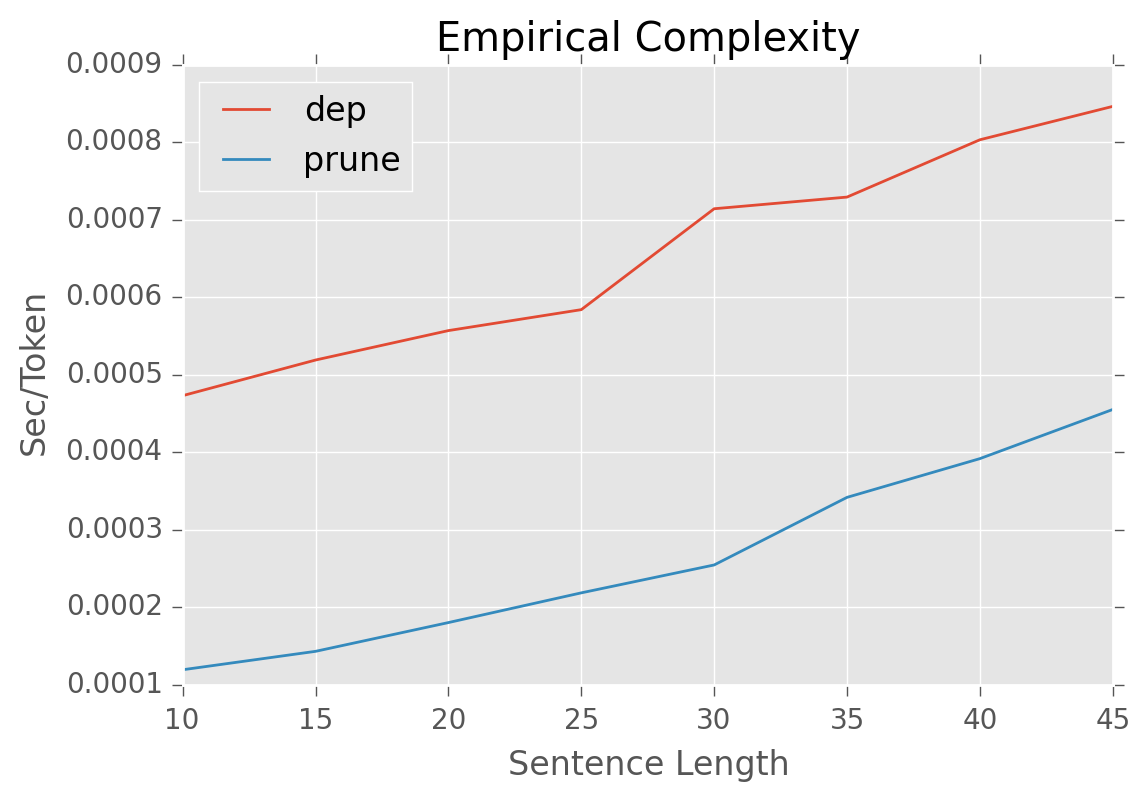
\includegraphics[scale=0.4]{../notebooks/comp}
  \label{tab:speed}
  \caption{Experiments of parsing speed. (a) The speed of the parser on its own and with pruning. (b) The end-to-end speed of the parser when combined with different dependency parsers. }
\end{table}




\section{Conclusion}

With recent advances in statistical dependency parsing, state-of-the-art parsers
have reached the comparable  dependency accuracy as the best phrase structure parsers. However,
these parser cannot be directly used in applications that require phrase-structure prediction. In this work
we have described a simple parsing algorithm and structured prediction system for this comparison, and show that it
can produce phrase-structure parses at comparable accuracy to state-of-the-art system.

One question for future work is whether these results are language
dependent, or whether these transformation can be projected across
languages. If this were possible, we could use a system of this form to learn phrase
structure parsers on languages with only dependency annotations.





\appendix{}

\section{Proof of PS Size}
\label{app:proof}

Consider the LCFG grammar with two rules $A = \RuleA{X}{X}{X}$ and  $ B = \RuleB{X}{X}{X}$ and a sentence $x_1, \ldots, x_{2n+1}$. Let the dependency parse be defined as $d_{n+1} = 0$ and $d_i = n+1$ for all $i \neq n + 1$, i.e.

\begin{center}

\scalebox{0.5}{
\begin{dependency}[theme=simple]
  \begin{deptext}[column sep=0.7cm]
    $1$ \& $2$ \& \ldots \& $n+1$ \& $\ldots$ \& $2n$ \& $2n+1$ \\
  \end{deptext}
  \deproot{4}{ROOT}
  \depedge{4}{1}{}
  \depedge{4}{2}{}
  \depedge{4}{6}{}
  \depedge{4}{7}{}
\end{dependency}
}
\end{center}

\noindent Since all rules have $h = x_n$ as head, a parse is a chain of $2n$ rules with each rule in $\{A, B\}$, e.g. the following are $BB...$, $BA...$, $AA...$

\begin{center}

\scalebox{0.6} {
\Tree [ .X $x_1$ [ .X $x_2$  [ .$\vdots$ $x_{n+1}$ ]   ] ]
\Tree [ .X $x_1$ [ .X  [ .$\vdots$ $x_{n+1}$ ] $x_{2n+1}$  ] ]
\Tree [ .X  [ .X  [ .$\vdots$ $x_{n+1}$ ]   $x_{2n}$ ] $x_{2n+1}$ ]
}
\end{center}


\noindent Since there must be equal $A$s and $B$s and all orders are possible, there are $2n \choose n$ valid parses and $|\mathcal{Y}(x, d)|$ is $O(2^n)$.
% \textbf{Acknowledgment} sections should go as a last (unnumbered) section immediately
% before the references.



\bibliography{full}
\bibliographystyle{naaclhlt2015}

\end{document}

%%% Local Variables:
%%% mode: latex
%%% TeX-master: t
%%% End
